%!TEX root = pfc-memoria.tex
%!TEX encoding = UTF-8 Unicode

\chapter{Planificación}

\epigraph{``El progreso no se consigue por la suerte o por accidente sino trabajando en uno mismo diariamente.''}{\textsc{Epictetus} (55--135)}

En este capítulo organizaremos el desglose de tareas para hacer una planificación de las mismas en el calendario.

\section{Metodología de trabajo}

Utilizaremos un modelo de ciclo de vida iterativo en espiral \citep{Boehm1988}, pero dividiendo el proceso en dos paquetes de trabajo:
\begin{enumerate}[WP1]
\item La lectura y estudio de la bibliografía sobre NLP y ML; y su parte de documentación en la memoria.
\item Estudio de bibliotecas y frameworks disponibles para la construcción del GUI; y análisis, diseño, implementación y pruebas del software; y su parte de documentación en la memoria.
\end{enumerate}

\begin{figure}[htbp]
\centering
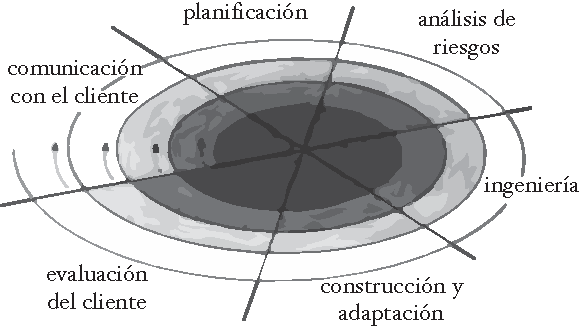
\includegraphics[width=0.58\textwidth]{espiral}
\caption[Modelo de ciclo de vida en espiral]{Modelo de ciclo de vida en espiral \citep{Boehm1988}}
\label{fig:espiral}
\end{figure}

El tutor de proyecto, que hace de cliente, recibió aproximadamente una comunicación cada semana y media o dos semanas, durante junio y julio, con el progreso de la memoria por capítulos.

\section{Herramientas utilizadas}

Para la elaboración de la memoria, utilizamos el sistema de composición tipográfica \XeLaTeX. Para el retoque de imágenes, y de ilustraciones: Adobe Photoshop y Adobe Illustrator. Para la gestión bibliográfica usamos la aplicación Mendeley.

Como gestor de código fuente: \codet{git} en local, y el servicio de Bitbucket\footnote{\url{https://bitbucket.org}} como respaldo.

Para la codificación en Python, usamos el IDE de Jetbrains PyCharm.

\section{Planificación y coste}

El desglose de tareas se puede ver en la \autoref{tbl:tareas}. Para el cálculo, se ha estimado un día de trabajo de 8 horas, y una semana de 5 días, de lunes a viernes. Se estimó inicialmente un esfuerzo necesario de \framebox[2cm]{15w~3d~4h}, al que hay que sumar un retraso de \framebox[2cm]{1w~3d~0h} por los problemas con el framework Kivi~1.9, y en la implementación de la tabla de datos en QML. Estos dos problemas se comentarán más adelante en el \fullref{chap:implementacion}.

Por lo tanto, se ha realizado un trabajo final de \SI{680}{horas}, aunque lo estimado fueron \SI{628}{horas}. Suponiendo un precio presupuestado de \SI{9}{€/hora}:
\[
\SI{628}{horas} \times \SI{9}{€/hora} \; = \; \SI{5652}{€} 
\]

\begin{table}[htbp]
\centering
\csvautotabular{gantt.csv}
\caption{Listado de tareas del proyecto}
\label{tbl:tareas}
\end{table}

Se puede ver un diagrama de Gantt con el calendario de las tareas en las figuras \ref{fig:gantt1} y \ref{fig:gantt2}.

\begin{landscape}
\begin{figure}[htbp]
\centering
\vspace*{0.6cm}
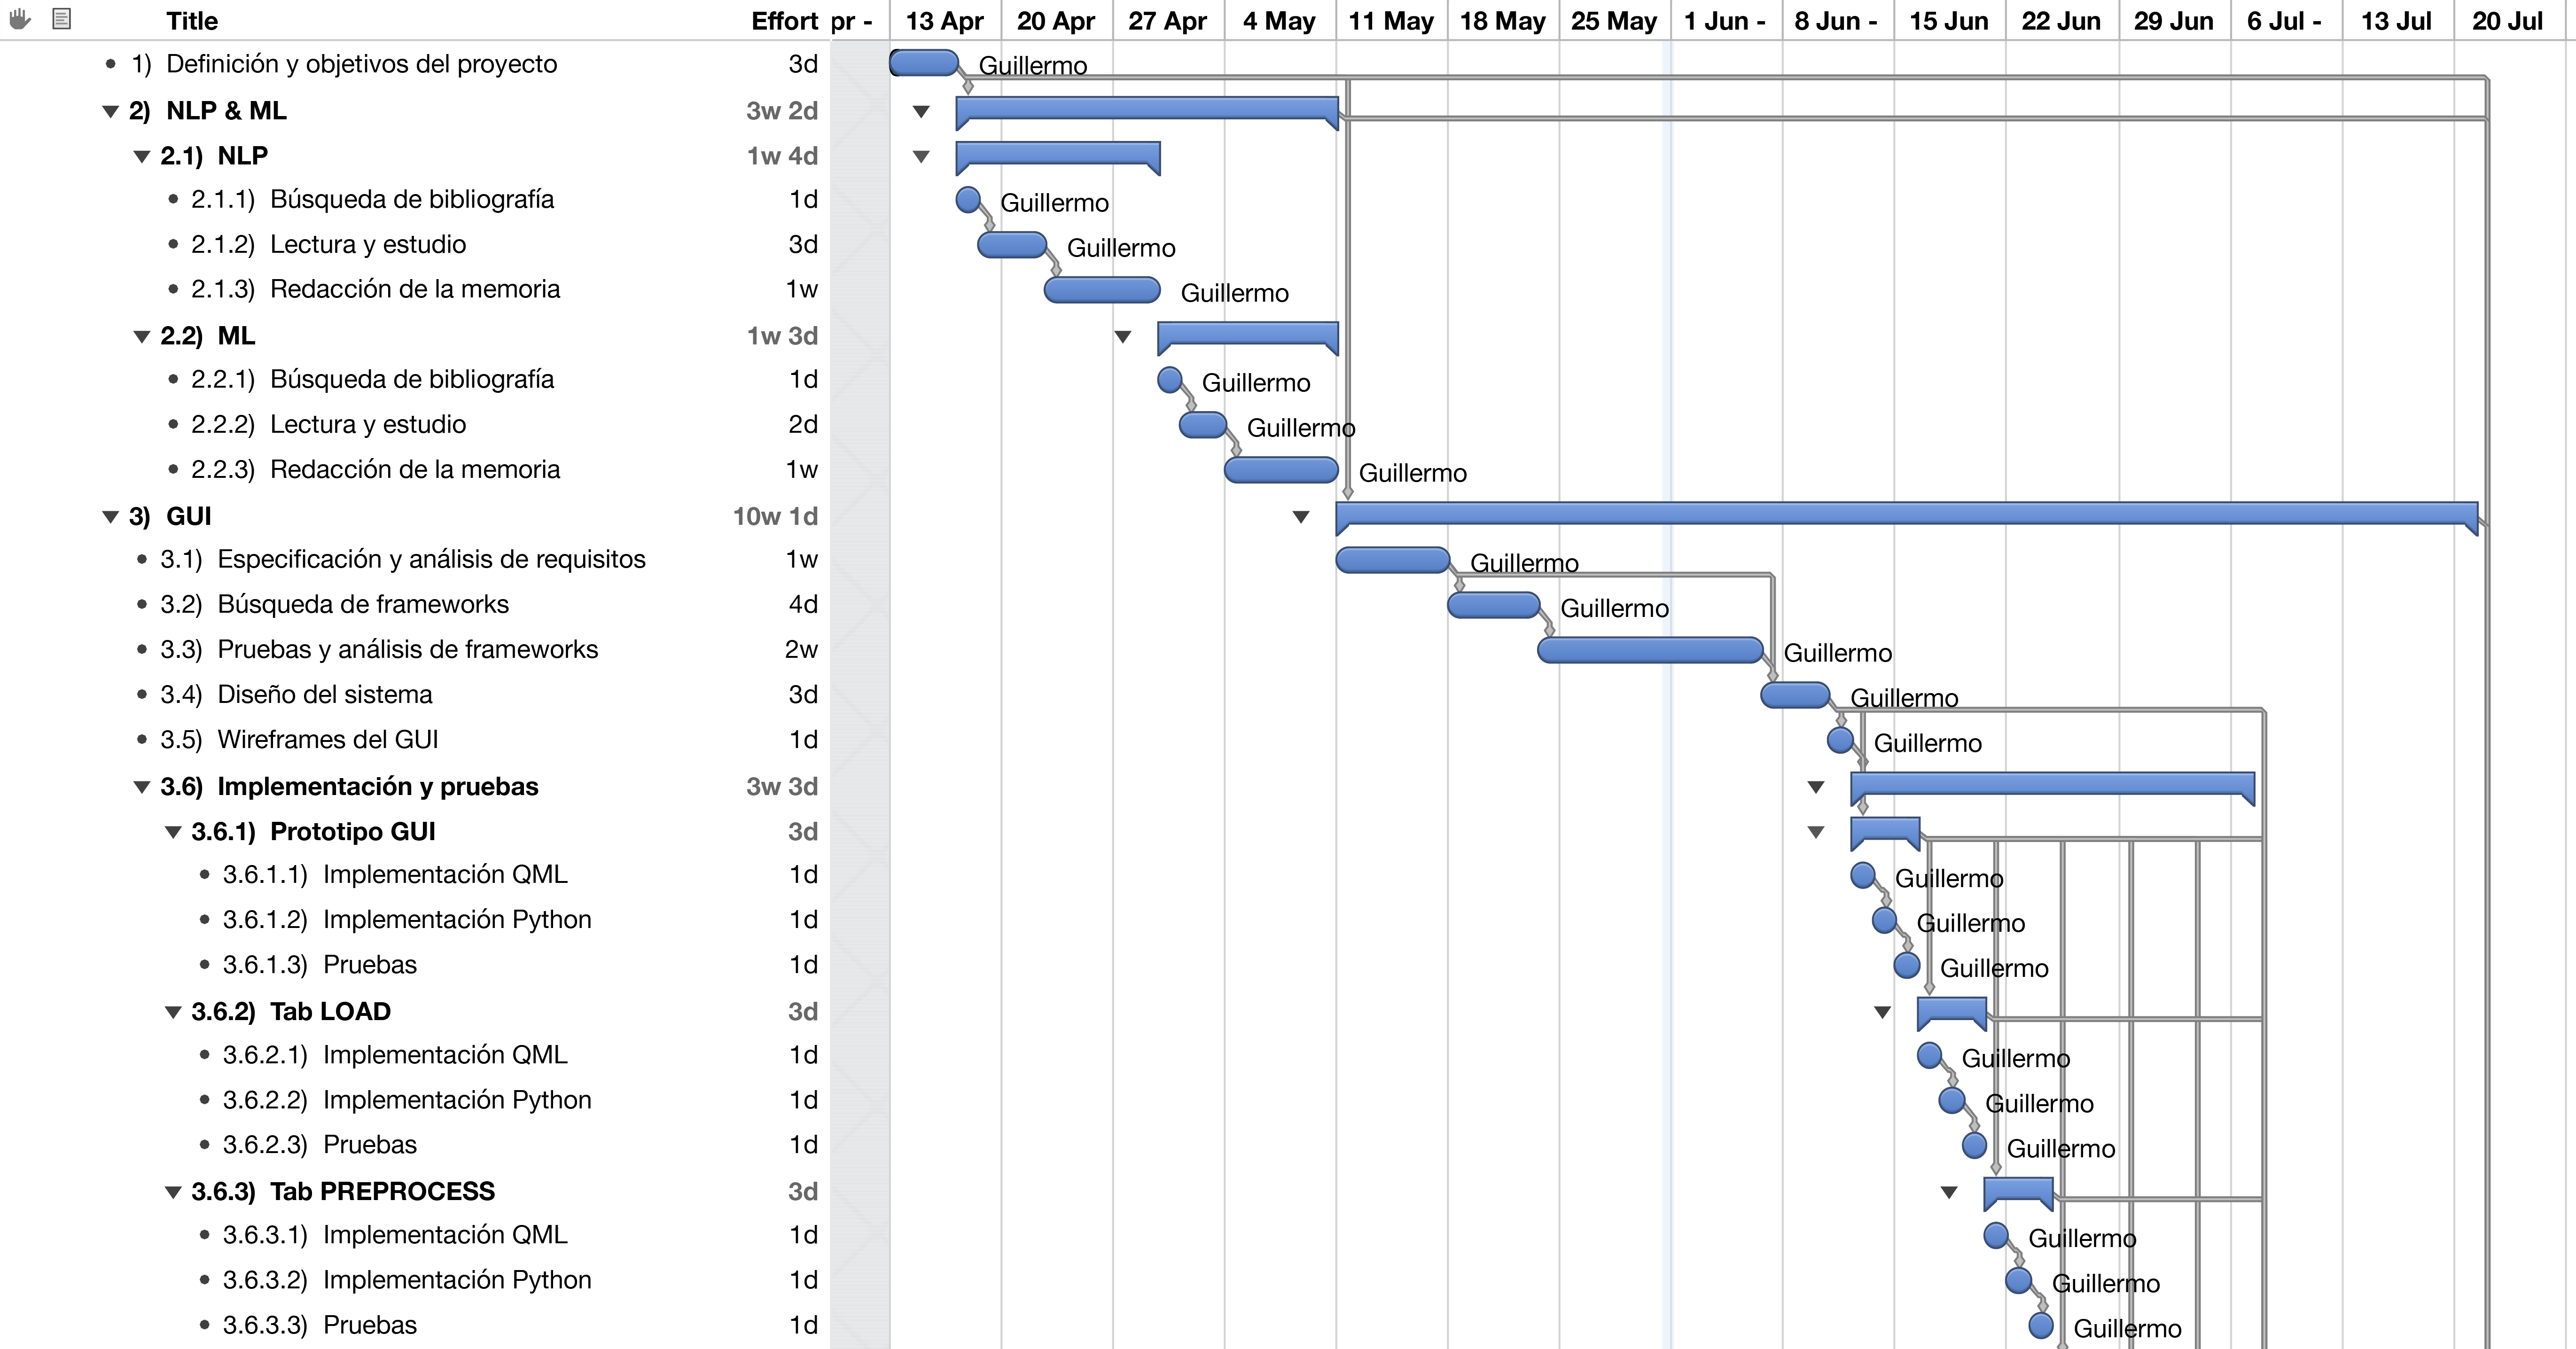
\includegraphics[width=24cm]{gantt1}
\caption{Cronograma (I)}
\label{fig:gantt1}
\end{figure}
\end{landscape}

\begin{landscape}
\begin{figure}[htbp]
\centering
\vspace*{1.2cm}
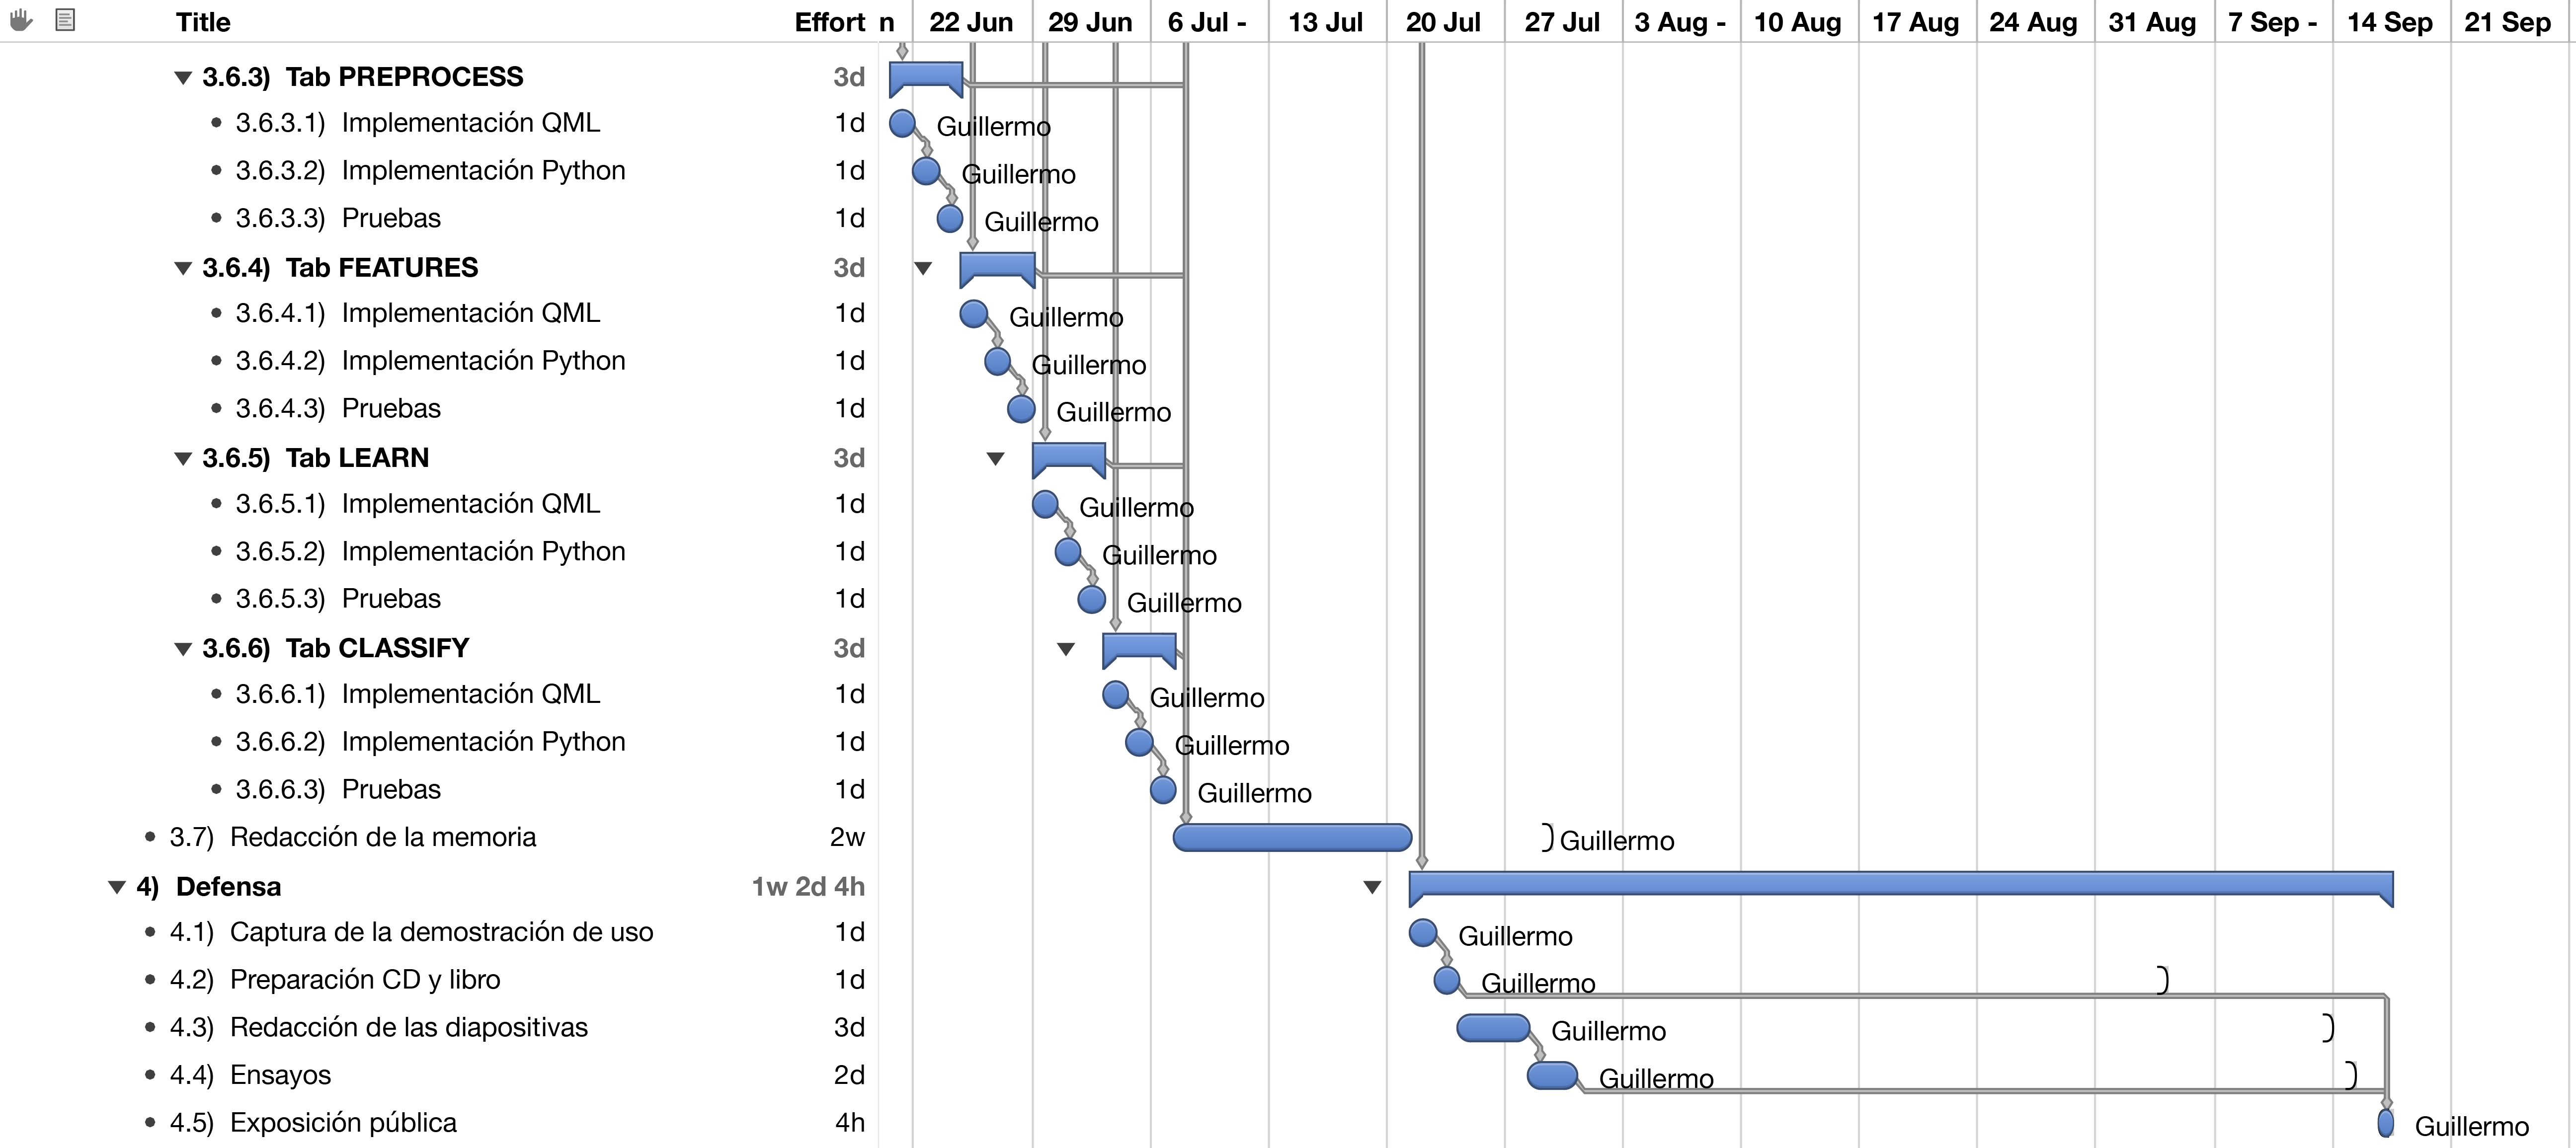
\includegraphics[width=24cm]{gantt2}
\caption{Cronograma (y II)}
\label{fig:gantt2}
\end{figure}
\end{landscape}
